\documentclass[11pt,a4paper]{article}
% rozmery stranky
\usepackage[left=1.5cm,text={18cm, 25cm},top=2.5cm]{geometry}
% cestina a fonty
\usepackage[czech]{babel}
\usepackage[utf8]{inputenc}
\usepackage[T1]{fontenc}
% dalsi balicky
\usepackage{graphicx}
\usepackage{enumitem}
\usepackage{indentfirst}
\usepackage{float}
\usepackage{url}
\usepackage[bookmarksopen,colorlinks,plainpages=false,urlcolor=blue,
unicode,linkcolor=black]{hyperref}


\begin{document}

  \begin{titlepage}
    \begin{center}
      \Huge
      \textsc{Fakulta informačních technologií\\ Vysoké učení technické v~Brně}
      \vspace{100px}
      \begin{figure}[!h]
        \centering
        
\includegraphics[height=5cm]{logo.jpg}
      \end{figure}
      \\[50mm]
      \LARGE{Studie účelnosti zbudování vodní cesty Dunaj-Odra-Labe \,--\, 
             zadání č. 2}
      \vfill
    \end{center}
    \Large{Roman Blanco (xblanc01) \hfill 7.12.2014 \\
           Adam Jež (xjezad00)}
  \end{titlepage}

  \tableofcontents
  \newpage

  \section{Úvod}

    Cílem zadaného projektu bylo prostudovat zdroje, zabývající se účelností
    vybudování vodního koridoru Dunaj-Odra-Labe, a podle zjištěných údajů
    stanovit kvalifikovaný odhad roční poptávky po lodní přepravě mezi
    zvolenými uzly. 

    Součástí zadání bylo také navrhnout a implementovat model SHO
    (Systém hromadné obsluhy -- IMS přednášky \ref{peringer} slide č. 139)
    dopravní cesty, včetně
    stavebních prvků.

    \subsection{Autoři}

      Autory projektu jsou Roman Blanco (xblanc01) a Adam Jež (xjezad00) \,--\,
      studenti 3. ročníku bakalářského studia na Fakultě Informačních
      technologii VUT v Brně. Prioritním zdrojem informací týkajících se
      zadaného tématu byly veřejně přístupné zdroje. Některé informace nám
      byly poskytnuty autory projektu zabývajícího se výstavbou koridoru.

    \subsection{Ověřování validity modelu}

      Ověřování validity modelu probíhalo pomocí experimentů, a to simulací ve
      virtuálním prostředí (Validace modelu -- IMS přednášky \ref{peringer}
      slide č. 37). Ověřovalo se, zda modelová situace odpovídá reálné situaci,
      přičemž informace byly čerpány pouze z věrohodných zdrojů.
      Jelikož reálný systém, určený simulovaným modelem, v současné době
      neexistuje, jako validní jsme model prohlásili na základě
      informací získaných z těchto zdrojů.

  \section{Rozbor tématu}

    Informace, potřebné pro úspěšnou implementaci byly vyhledány na veřejně
    přístupných stránkách na internetu. Problémem při využívání těchto zdrojů
    byla skutečnost, že mnoho informací, bylo uvedeno pouze v sumarizovaných
    hodnotách za období celého roku.  Pro některé hodnoty tak musel být použit
    kvalifikovaný odhad, podpořený údaji čerpanými ze statistik a dalších
    databází. Mimo již zmíněných veřejně přístupných webových stránek nám také
    často jako zdroj údajů posloužily diplomové či bakalářské práce. Níže je
    uveden souhrn hodnot, které jsme tímto způsobem získali:

    \noindent
    Hodnoty týkající se plavební komory:

    \begin{itemize}
      \item doba uzavření vrat plavební komory je 60 sekund
      \item doba otevření vrat plavební komory je 30 sekund
      \item doba vplutí do plavební komory je 516 sekund
      \item doba vyplutí z plavební komory je 355 sekund
      \item nízká plavební komora je taková, u níž výškový rozdíl mezi
            hladinami toku před a za komorou není větší než 12.5 m.
            Pokud plavební komora vyrovnává výšku hladiny přesahující 12.5 m,
            nazýváme ji vysokou plavební komorou
      \item napuštění nebo vypuštění 1 výškového metru nízké plavební komory
            odpovídá doba 40 s
      \item napuštění nebo vypuštění 1 výškového metru  vysoké plavební komory
            odpovídá doba 25,45 s
    \end{itemize}

    \noindent
    Hodnoty týkající se plavby v tunelu:

    \begin{itemize}
      \item bezpečná rychlost lodi při plavbě v tunelu je 2,22 m/s

      \item hranice, kdy se začne aplikovat seskupování je 3470 m
            (Studie projektu \ref{studie} -- stana č. 48).
    \end{itemize}

    \noindent
    Hodnoty týkající se plavby v akvaduktu:

    \begin{itemize}
      \item rychlost při plavbě v tunelu je 2,77 m/s
      \item hranice, kdy se začne aplikovat seskupování je 2090 m
    \end{itemize}

    \break

    \noindent
    Obecné hodnoty při plavbě:

    \begin{itemize}
      \item rychlost plavby v kanálu je 3,33 m/s
      \item rychlost plavby po proudu toku řeky je 4,16 m/s
      \item rychlost plavby proti proudu toku řeky je 1,66 m/s
      \item maximální náklad lodi je 4000 tun
    \end{itemize}

    \noindent
    Dále jsme také pracovali s těmito informacemi:

    \begin{itemize}
      \item tunely jsou navrhovány jako jednolodní, tedy lodi v tunelu se
            nemohou pohybovat proti sobě. Lodě, které se chystají projet
            tunelem stejným směrem se mohou seskupit za účelem zrychlení plavby
            (Kniha \ref{kniha} -- strana č. 157)
      \item je plánovaná vodní třída Vb, kde mohou plout motorové nákladní lodě
            o nosnosti 2500 tun, nebo menší řičně-námořní lodě a tlačné
            soupravy s nosností 4000 tun
            (Kniha \ref{kniha} -- strana č. 136)
      \item provoz plavebních komor je 24 hodin denně
            (Studie projektu \ref{studie} -- strana č. 38)
    \end{itemize}
        
    Velmi dobrým zdrojem informací o plánované trase koridoru byly materiály
    volně dostupné na internetové stránce projektu, který se problematikou
    vodního koridoru Dunaj-Odra-Labe dlouhodobě intenzivně zabývá, a také
    literatura \ref{kniha}, kterou nám poskytli její autoři.

    \subsection{Popis použitých postupů}

      V literatuře i na webových stránkách byly zobrazeny všechny části
      plánovaného koridoru s potřebnými údaji o trase:
      \begin{itemize}
        \item délky tunelů
        \item délky akvaduktů
        \item výškové rozdíly u plavebních komor
      \end{itemize}

      V knize byl také údaj určující, na kolikátém kilometru se stavební prvky
      nachází, z čehož bylo možné určit vzdálenosti mezi těmito prvky a tedy i
      délky úseků řek. (obrazek. č 1).  Označeny nebyly pouze polohy přistavů,
      tedy přibližná poloha přistavů byla odhadnuta pomocí blízkých stavebních
      prvků.

    \begin{figure}[ht!]
      \centering
      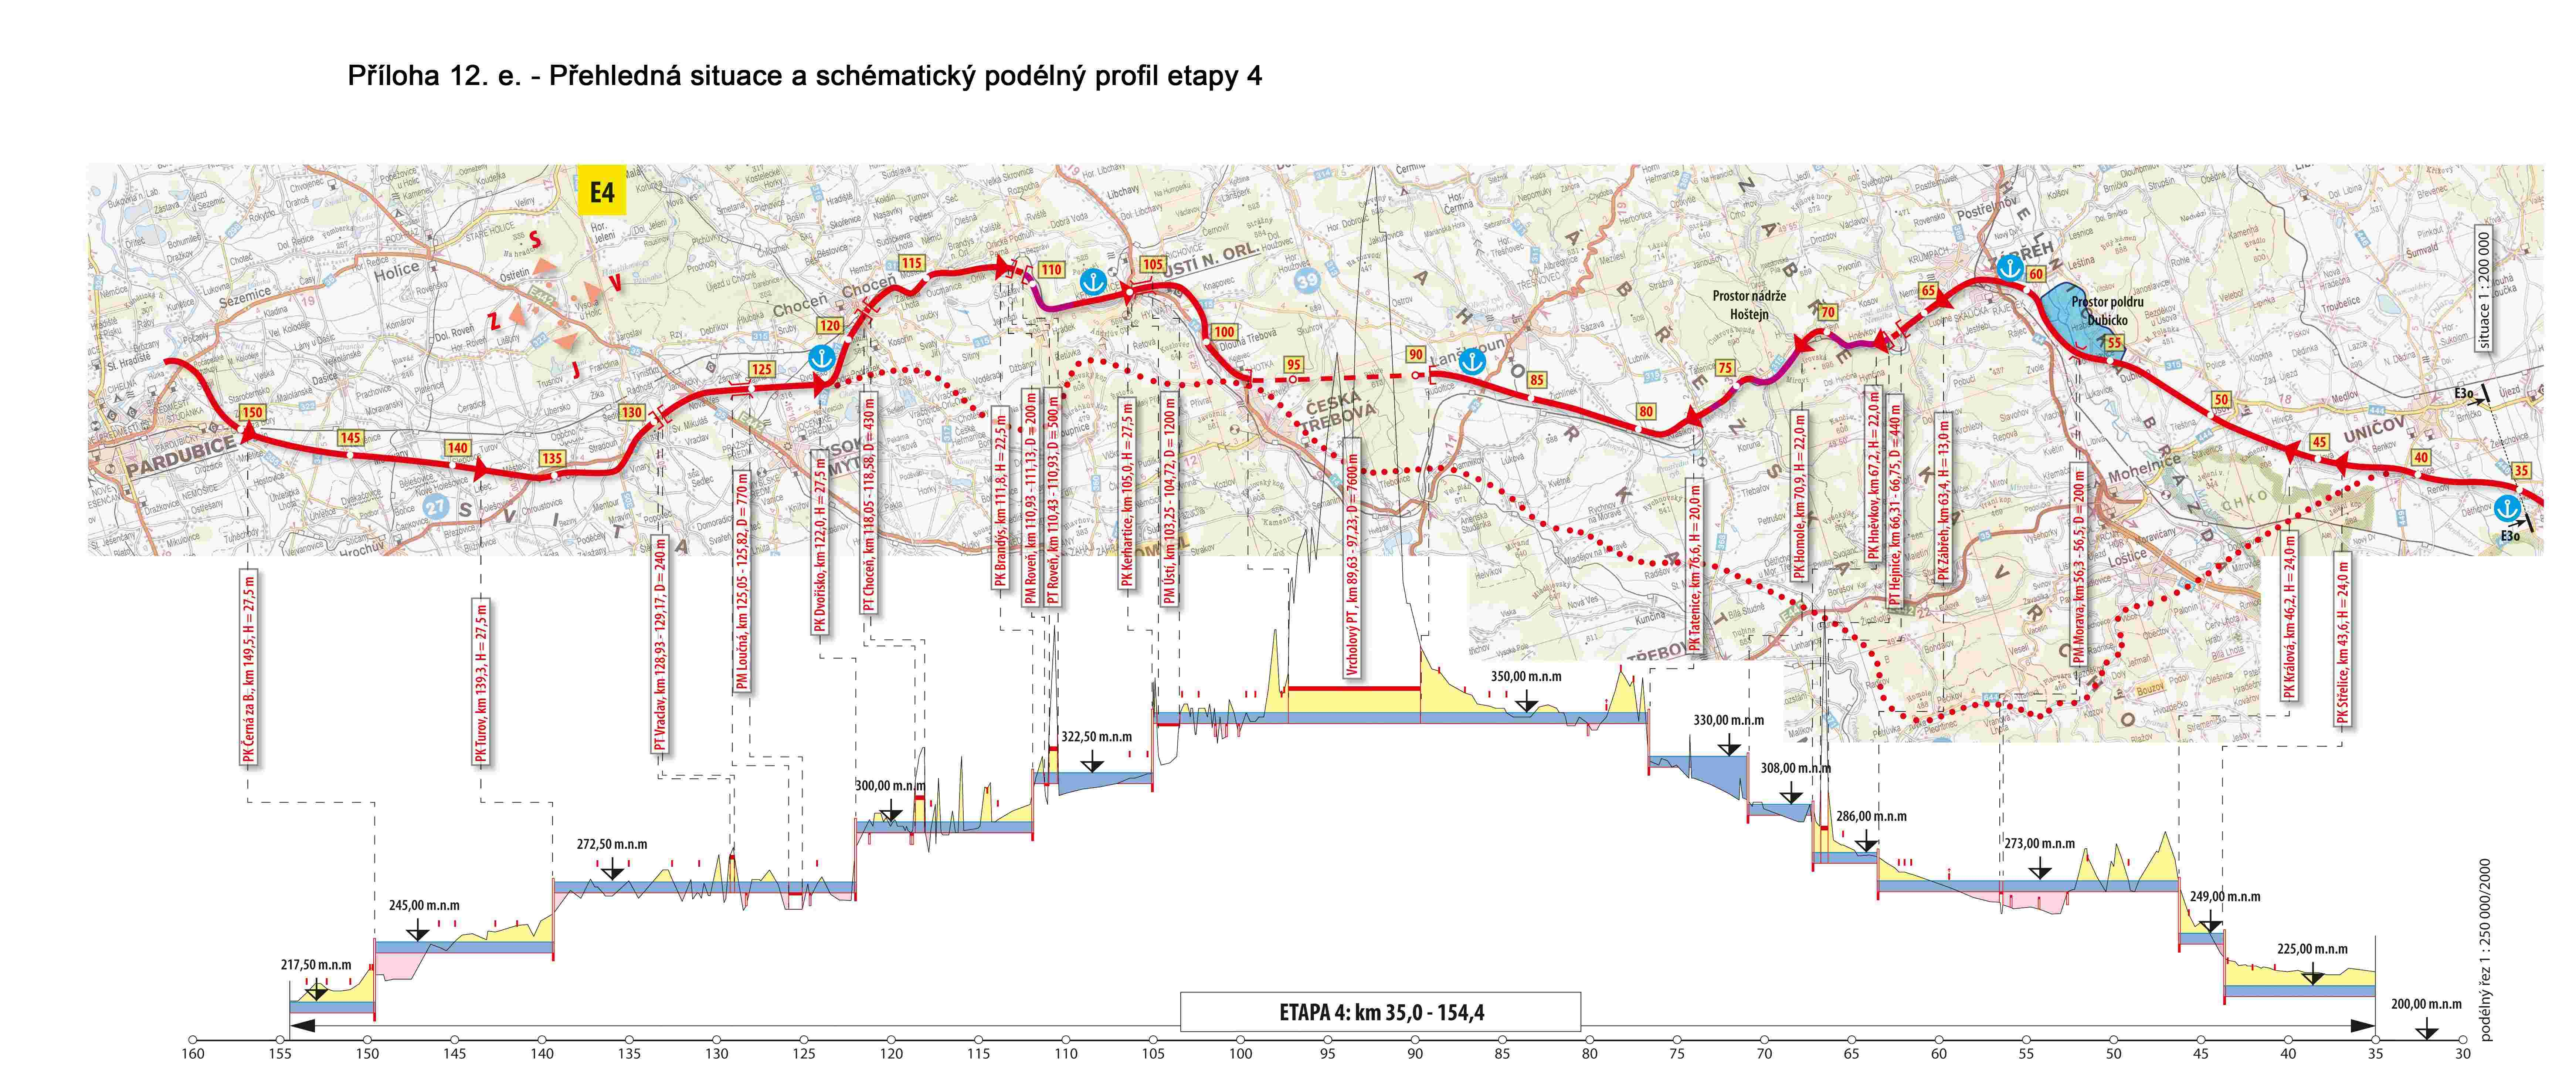
\includegraphics[width=1\textwidth, natwidth=6969, natheight=2953]
                      {etapa4.jpg}
      \caption{Ukázka jedné etapy koridoru z poskytnuté literatury
      \label{overflow}}
    \end{figure}

    \subsection{Popis použitých technologií}

      \begin{itemize}
        \item C++ \href{http://www.cplusplus.com/}{cplusplus.com}
        \item SIMLIB
          \href{http://www.fit.vutbr.cz/~peringer/SIMLIB/}
               {www.fit.vutbr.cz/\textasciitilde peringer/SIMLIB/}
        \item g++ \href{http://www.cprogramming.com/g++.html}
                       {www.cprogramming.com/g++.html}
        \item GNU/Linux, distribuce Fedora, Ubuntu
          \href{http://fedoraproject.org}{fedoraproject.org/},
          \href{http://ubuntu.com}{ubuntu.com}
      \end{itemize}

  \section{Koncepce modelu}

    \subsection{Forma konceptuálního modelu}


      Petriho síť na obrázku č. \ref{petri_1} zobrazuje mechanismus proplutí
      tunelem (stejný mechanismus lze aplikovat při proplouváníí mostu).
      Proměnná \texttt{M} udává počet lodí, které mohou vplout do tunelu zároveň.
      Ve téměř všech tunelech je tato proměnná rovna $1$. Výjimkou je tunel
      \textit{Vrcholový}, a to kvůli své délce \,--\, 7600 metrů. U tohoto
      tunelu je proměnná \texttt{M} nastavena na hodnotu $3$
      
      a to zejména kvůli blízkým plavebním komorám. Nastavení vyšší proměnné
      tak sníží časovou ztrátu lodí při následném překonávání plavebních komor.
      Hodnota je určena na základě tabulky ve
      studii (Studie projektu \ref{studie} -- stana č. 48).

      \begin{center}
        \begin{tabular}{| l | l | l | l | l | l | l | l |}
          \hline
          počet lodí v závěsu & 1 & 2 & 3 & 4 & 5 & 6 & 7 \\ \hline
          $L_{mez}$ pro jednoduché pl. k. $(km)$
            & 3,47 & 6,94 & 10,42 & 13,89 & 17,36 & 20,83 & 24,30 \\ \hline
          $L_{mez}$ pro dvojité pl. k. $(km)$
            & 1,63 & 3,26 &  4,88 &  6,51 &  8,14 &  9,77 & 11,40 \\ \hline
          \end{tabular}
      \end{center}

      Proměnná \texttt{T} udává čas potřebný k proplutí tunelu.
      Tento čas je určený délkou tunelu a bezpečnou
      rychlostí v těchto jednolodních tunelech, která činí
      8 km/h (Studie projektu \ref{studie} -- strana č. 47, poznámka pod čarou).
      Pro jednoduchost byl v petriho síti zanedbán mechanismus, který je pro správné
      fungování simulace nutný \,--\, timeout. Po určité době bez proplutí lodě
      se směr tunelu automaticky změní. Doba byla navržena jako dvojnásobek
      proplouvací doby.

      \begin{figure}[H]
        \centering
        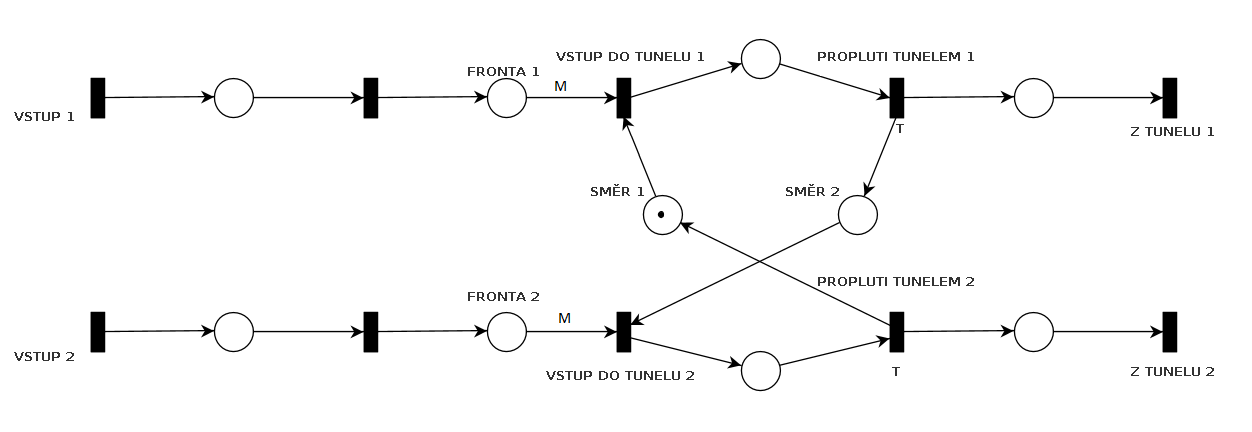
\includegraphics[width=1\textwidth, natwidth=940, natheight=325]
                        {petri_net_1.png}
        \caption{Petriho síť proplutí tunelu} \label{petri_1}
      \end{figure}

      \break

      Petriho síť na obrázku č. \ref{petri_2} zobrazuje mechanismus proplutí
      plavební komorou. Proměnná \texttt{X} určuje čas, za který:

      \begin{enumerate}
        \item loď vpluje do komory
        \item zavřou se vrata komory
        \item naplní se komora
        \item otevřou se vrata
        \item loď vypluje z komory
      \end{enumerate}

      Kromě naplnění komory jsou všechny konstanty získané ze
      studie[3] (Studie projektu - strana č.46-47).
      Doba napuštění (popř. vypuštění \,--\, časy jsou totožné) se odvíjí od
      výšky, kterou komora pomáhá překonávat. Doba naplnění jednoho metru v
      komoře byla zjištěna ze studie[3] (Studie projektu - strana č. 44).
      Rozlišuje se také mezi vysokými a nízkými plavebními komorami.
      Ve vysokých komorách se může voda plnit rychleji.
      Proměnná \texttt{T} udává čekací dobu, po kterou, pokud není plavební
      komora nijak využita, je komora přečerpána kvůli čekajícímu plavidlu na
      opačné hladině, než je aktuální hladina komory. Hodnotu proměnné 
      \texttt{T} jsme určili experimentováním.

      \begin{figure}[H]
        \centering
        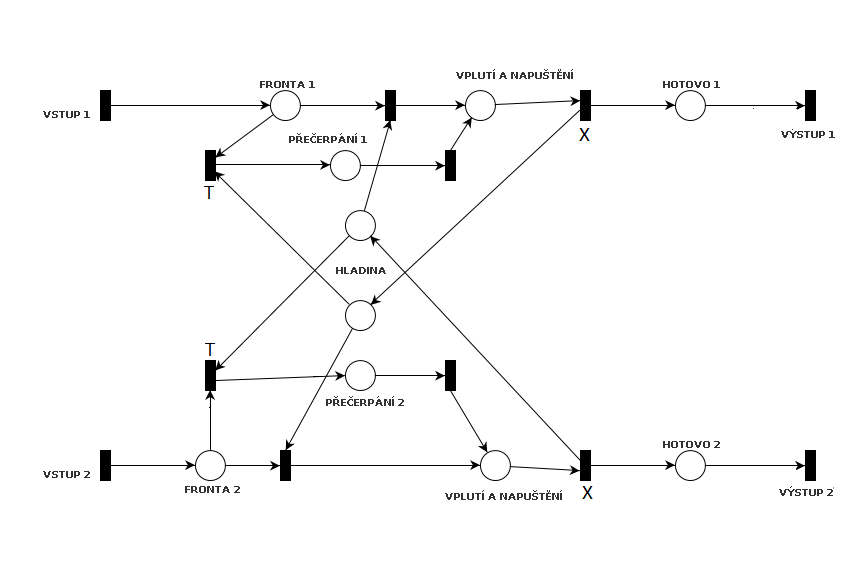
\includegraphics[width=1\textwidth, natwidth=940, natheight=325]
                        {petri_net_2.png}
        \caption{Petriho síť proplutí plavební komorou \label{petri_2}}
      \end{figure}

  \section{Architektura simulačního modelu}

    Následující kapitola pojednává o implementační části projektu. Pro pochopení
    implementace je potřeba mít alespoň minimální znalosti jazyka C++ a 
    objektově orientovaného programování.
    K umožnění experimentů s realným systémem bylo nejprve nutno z nabytých znalostí
    vytvořit abstraktní model a poté simulační model (Princip Modelování a 
    simulace -- IMS přednášky \ref{peringer} slide č. 9-10).

    \subsection{Návrh objektově orientovaného modelu}
    
      Všechny prvky (stavební prvky, řeka), které mají značný časový vliv na
      dobu plavby lodě, mají svou vlastní třídu.

      \begin{itemize}
        \item třída \texttt{WaterItem} \\
              jedná se o abstraktní třídu, z níž jsou zděděny všechny prvky
              vodní cesty. Třida se stará o odchytávání statistik pomocí metod
              \texttt{Start} a \texttt{End}. Dále třida obsahuje dvě fronty 
              -- každá fronta pro jeden směr plavby.

              Rozhraní třídy výžaduje implementaci metod \texttt{getType} a 
              \texttt{getLegth}. Sémantikou metody \texttt{getType} je vracení
              typu prvku vodní cesty, \texttt{getType} analogicky vrací jejich 
              délky.

        \item třída \texttt{Chamber} \\
              tato třída je abstrakcí plavební komory. 
              Dědí výše popisovanou třídu \texttt{WaterItem}.

              Metody implementované v ní jsou \texttt{seize}, \texttt{release}
              a \texttt{performAction}. 

              Metoda \texttt{seize} se stará o povolení vjezdu lodi do plavební
              komory a zabránění dalším lodím využít komoru ve chvíli kdy je
              obsazena. Pokud se hladina plavební komory neshoduje s hladinou
              po které přijíždí loď, je loď zařazena do fronty a je nastaven
              timeout, po jehož uplynutí se plavební komora naprázdno přečerpá,
              pokud není do doby vypršení timeoutu plavební komora využita.
              Metoda \texttt{performAction} vykoná úkon vplutí do komory,
              napuštění komory a vyplutí z ní.

              Hodnota timeout nebyla ve zdrojích nalezena, a bylo nutno ji
              odhadnout na základě experimentů. Hodnota je dvojnásobkem doby
              pro proplutí plavební komorou.

              U dalších tříd je účel této metody stejný.

              Metoda \texttt{release} zařídí případné aktivování dalšího
              plavidla ve frontě.
        \item třídy \texttt{Tunel} a \texttt{Bridge} \\
              také obsahuje metody \texttt{seize}, \texttt{performAction} a
              \texttt{release}. Rozdíl u metody \texttt{seize} je, že lodě se
              střídají v proplouvání tunelem. Na základě délky tunelu
              (či mostu) se lodě seskupují.
        \item třídy \texttt{Channel}, \texttt{Port} a \texttt{River} \\
              třídy implementují pouze metodu \texttt{performAction}, v níž se
              počítá doba proplutí daným místem. Speciálně u třídy
              \texttt{River}, která je abstrakcí tekoucí řeky, jsme brali v
              úvahu i směr toku.
        \item třída \texttt{CargoShip} \\
              Dědí od třídy \texttt{Process} z knihovny SIMLIB. Implementuje
              metodu \texttt{behaviour}, ve které podle typu právě
              proplouvaného prvku vyvolá odpovídající akci. Objekt této třídy
              má daný počáteční i
              koncový uzel symbolizující přístav.
      \end{itemize}

    \subsection{Načítání trasy a transportovaného objemu}

      Třídy načítají údaje o trase ze zdrojových souborů ve složce
      \textit{input.}

      V souboru \textit{info.tsv} jsou uloženy informace o všech 
      prvcích vodní trasy. Typ každého prvku je určen identifikátorem, podle
      něhož se dále rozhoduje o zpusobu zacházení se souvisejícími údají.

      V souboru \textit{connections.tsv} jsou dvojice identifikátorů jejichž
      prvky se nachází v trase bezprostředně za sebou.

      Dále jsou zde konfigurační soubory, které určují trasu a převezený objem
      za rok. Jednotkou je 1000 tun.

  \section{Podstata simulačních experimentů a jejich průběh}

    Za cíl jsme si stanovili zjistit propustnost simulovaného vodního koridoru.
    Simulovali jsme 3 různé scénáře a porovnáním zjišťovali jejich vliv na časovou
    náročnost dané trasy

    \break

    \noindent 
    Scénář TREND -- Prognóza objemu přepravy (Analýza hospodářského
    potenciálu \ref{analyza} -- strana č. 226)
    \begin{center}
      \begin{tabular}{| l | l | l |}
        \hline
        & rok 2020 & rok 2050 \\ \hline
        Hodonín - Otrokovice & 7470 tis. t & 10280 tis. t \\ \hline
        Otrokovice - Přerov & 7600 tis. t & 14600 tis. t \\ \hline
        Přerov - Mošnov &  8100 tis. t & 11150 tis. t \\ \hline
        Mošnov - Ostrava & 6520 tis. t & 8970 tis. t \\ \hline
        Přerov - Olomouc & 4850 tis. t & 6680 tis. t \\ \hline
        Olomouc - Pardubice & 4740 tis. t & 6530 tis. t \\ \hline
        \end{tabular}
    \end{center}

    \noindent 
    Scénář VYSOKÝ -- Prognóza objemu přepravy (Analýza hospodářského
    potenciálu \ref{analyza} -- strana č. 230)
    \begin{center}
      \begin{tabular}{| l | l | l |}
        \hline
        & rok 2020 & rok 2050 \\ \hline
        Hodonín - Otrokovice & 9730 tis. t & 14660 tis. t \\ \hline
        Otrokovice - Přerov & 9710 tis. t & 14620 tis. t \\ \hline
        Přerov - Mošnov & 10020 tis. t & 15090 tis. t \\ \hline
        Mošnov - Ostrava & 9890 tis. t & 14900 tis. t \\ \hline
        Přerov - Olomouc & 5820 tis. t & 8770 tis. t \\ \hline
        Olomouc - Pardubice & 5610 tis. t & 8450 tis. t \\ \hline
        \end{tabular}
    \end{center}

    \noindent 
    Scénář NÍZKÝ -- Prognóza objemu přepravy (Analýza hospodářského
    potenciálu \ref{analyza} -- strana č. 230)
    \begin{center}
      \begin{tabular}{| l | l | l |}
        \hline
        & rok 2020 & rok 2050 \\ \hline
        Hodonín - Otrokovice & 5170 tis. t & 6340 tis. t \\ \hline
        Otrokovice - Přerov & 5260 tis. t & 6450 tis. t \\ \hline
        Přerov - Mošnov & 5610 tis. t & 6880 tis. t \\ \hline
        Mošnov - Ostrava & 4500 tis. t & 5530 tis. t \\ \hline
        Přerov - Olomouc & 3340 tis. t & 4090 tis. t \\ \hline
        Olomouc - Pardubice & 3260 tis. t & 4000 tis. t \\ \hline
        \end{tabular}
    \end{center}

  \section{Závěr}

  \section{Reference}

    \begin{enumerate}[label={[\arabic*]}]
      \item Peringer, P.: Modelování a simulace, Přednášky. Brno, Září 2014
        \label{peringer}
      \item Mapy s etapami výstavby koridoru \\
        \href{http://d-o-l.cz/index.php/cs/kestazeni/category/14}
        {http://d-o-l.cz/index.php/cs/kestazeni/category/14} \label{mapa}
      \item Studie projektu výstavby vodního koridoru D-O-L,
            Ministerstvo průmyslu a obchodu \\
        \href{http://d-o-l.cz/index.php/cs/kestazeni/category/6}
             {http://d-o-l.cz/index.php/cs/kestazeni/category/6} \label{studie}
      \item Analýza hospodářského potenciálu dopravního koridoru \\
        \href{http://d-o-l.cz/index.php/cs/kestazeni/category/27}
             {http://d-o-l.cz/index.php/cs/kestazeni/category/27} \label{analyza}
      \item Plánovaná trasa koridoru zaznačená v Google Maps \\
        \href{http://povode.aspone.cz/Maps/dol.html}
             {http://povodne.aspone.cz/Maps/dol.html} \label{google-mapa}
      \item Podzimek, J., : Křižovatka tří moří, Vodní koridor Dunaj-Odra-Labe,
            vydání 2., In:Hejkal, 2012, ISBN: 978-80-254-0105-7 \label{kniha}
    \end{enumerate}

  \appendix
  \newpage

  \section{Přílohy}

  \end{document}
